\documentclass[twocolumn,nofootinbib]{revtex4-1}
\usepackage{graphics}
\usepackage[caption=false]{subfig}
\usepackage{amsmath}
\usepackage{hyperref}
\usepackage{amssymb}
\usepackage{color}
\usepackage{epsfig}
\usepackage{latexsym}
\usepackage{tensor}
%\usepackage{wasysym}
\usepackage{comment}
%\usepackage{graphicx}
%\usepackage{psfrag}

\graphicspath{{poster/figures/}}

%\newcommand{\gw}{gravitational wave }
%\newcommand{\gws}{gravitational waves }
\newcommand{\subgw}{_{\textrm{\scriptsize{GW}}}}
\newcommand{\ee}[1]{\!\times\!10^{#1}}
\newcommand{\prob}{{\rm Pr}}
\newcommand{\grbrate}{{{\mathcal R}_{\mathrm{grb}}}}
\newcommand{\cbcrate}{{{\mathcal R}}}
\newcommand{\diff}{{\mathrm d}}
\newcommand{\rhostar}{{\rho^*}}
\newcommand{\dhor}{{\mathcal D}_{\mathrm{hor}}}

\def\imbh#1{intermediate mass black hole#1(IMBH#1)\gdef\imbh{IMBH}}
\def\smbh#1{supermassive black hole#1(SMBH#1)\gdef\smbh{SMBH}}
\def\bbh#1{binary black hole#1 (BBH#1)\gdef\bbh{BBH}}
\def\bns#1{binary neutron star#1 (BNS#1)\gdef\bns{BNS}}
\def\bh#1{black hole#1 (BH#1)\gdef\bh{BH}}
\def\ns#1{neutron star#1 (NS#1)\gdef\ns{NS}}
\def\gw#1{gravitational wave#1 (GW#1)\gdef\gw{GW}}
\def\sn#1{core-collapse supernova#1 (CCSN#1)\gdef\sn{CCSN}}
\def\pnw#1{post-Newtonian#1 (PN#1)\gdef\pnw{PN}}
\def\eos#1{equation of state#1 (EOS#1)\gdef\eos{EOS}}
\def\grb#1{gamma-ray burst#1 (GRB#1)\gdef\grb{GRB}}
\def\sgrb#1{short gamma-ray burst#1 (sGRB#1)\gdef\sgrb{sGRB}}
\def\amr#1{adaptive mesh refinement#1 (AMR#1)\gdef\amr{AMR}}
\def\isco#1{innermost stable circular orbit#1 (ISCO#1)\gdef\isco{ISCO}}
\def\cwb#1{Coherent WaveBurst#1 (CWB#1)\gdef\cwb{CWB}}
\def\mweg#1{Milky Way Equivalent Galaxy#1 (MWEG#1)\gdef\mweg{MWEG}}

\newcommand{\red}[1]{{\color{red}{#1}}}
\newcommand{\about}[1]{{\color{blue}{[THIS SECTION: #1]}}}
\newcommand{\add}[1]{{\color{magenta}{[TO INCLUDE: #1]}}}
\newcommand{\JC}[1]{{\color{magenta}{[[JC #1]]}}}
\newcommand{\placeholder}[2]{{\color{red}{[PLACEHOLDER](#1):}}{\color{red}{[}}#2{\color{red}{]}}}
\providecommand{\todo}[1]{{\color{red}$\blacksquare$~\textsf{[TODO: #1]}}}


%%%%%% Useful for draft editing
\usepackage{soul} 
\usepackage{ulem} \normalem 
\newcommand{\ec}[1]{{\noindent\color{red}{\it [[#1]] }}}
\newcommand{\laura}[1]{{\color{blue}{#1}}}
\newcommand{\LC}[1]{{\color{red}{[[LC #1]]}}}
\newcommand{\AB}[1]{{\color{blue}{[[AB #1]]}}}
\newcommand{\highlight}[1]{\colorbox{yellow}{#1}}
\newcommand{\simgt}{\mbox{$^{>}_{\sim}$}}

\begin{document}

\title{Constraints On Short, Hard Gamma-Ray Burst Beaming Angles From
Gravitational Wave Observations}
\author{James Clark, Ik Siong Heng, Martin Hendry}
\date{\today}

\begin{abstract}
\dots
\end{abstract}

\maketitle

\section{Introduction}

\about{Intro with also many words taken from search plans}

Extremely energetic bursts of gamma-rays from cosmological sources are observed by orbiting satellite detectors at a rate of about one per day. These extra-galactic events are generally referred to as GRBs.
GRBs are generally associated with systems which are also expected to be \gw{} sources: compact binary coalescences for \sgrb{}, with gamma-ray duration $<\!2\,$s and harder spectra [ref].

The detection of a GW signal in coincidence with a GRB would provide tremendous insight in the  astrophysics of these systems.
A merger signal associated to a short GRB would confirm the compact binary merger nature of the engine and allow for measurements of the binary components masses and spins, as well as constraints on the beaming angles and the neutron star equation of state.
However, it is only the observation of a GW signal that will conclusively show that the progenitor is a binary merger. While the merger scenario is preferred and at least one NS is required, both NS-NS and NS-BH progenitors are possible; GW observations will allow us to determine which of these it is. A population of GW-GRB observations will allow us to measure the fraction of GRBs associated with each progenitor type. The degeneracy between distance and inclination angle means that it will be difficult to measure the GRB beaming angle based on measurement of a single system. However, with observations of a population of binary merger sources, with and without GRB counterparts, we can constrain the average opening angle.   
A collection of joint short GRBs with redshift and GW measurements will also enable a relatively systematics-free measurement of the Hubble parameter at low redshift, which would provide constraints on cosmological models.

%It is common in the literature to draw inferences on the rate of binary
%coalescence $\cbcrate$, given some estimate for the beaming angle $\theta$ and
%the observed rate of \sgrb{s} $\grbrate$.  
In this work, we investigate what
statements can \emph{currently} be made on the beaming angle itself using the
upper limits placed on $\cbcrate$ from all-sky, all-time \gw{} searches and
explore the potential for direct inference of \sgrb{}  beaming angles in the
advanced detector era.

In this article, we first discuss the relationship between short gamma-ray bursts
and compact binary coalescences. In particular, we will focus on binary neutron 
star inspirals as the widely accepted progenitor for short gamma-ray bursts.
We then present our method for robustly inferring the jet opening angles of 
short gamma-ray bursts, using only gravitational wave observations. We 
demonstrate our method by assuming the nominal number of gravitational
wave signals observed from binary neutron star inspirals expected for
Advanced LIGO and Advanced Virgo in 2016 and 2022 as defined in [ref]. 
We also show that our approach can be used to place restrictions on the
short gamma-ray burst jet opening angle if there are no detections.
Finally, we conclude with a discussion on the implications of our work
as well as possible avenues for further extension of the work presented
here.

%\section{Inferring The sGRB Beaming Angle From Rate Measurements}
\section{Short gamma-ray bursts and compact binary coalescences}
\label{sec:sgrbs}

\about{Some description of BNS and how they are likely progenitors of short
gamma-ray bursts (This section describes our model and how sGRBs relate to BNS, currently with text taken from LVC search plans}

It is widely believed that compact binary coalescencesare the progenitors of \sgrb{s} [ref]. 
Observations of \sgrb{s} indicate that they are likely to result from mergers of binary systems consisting of  two neutron stars (\bns{}) or a neutron star and stellar mass ($< 10$ solar mass) black hole (NS-BH). 
At full sensitivity, they are potentially observable by advanced GW detectors to $\sim 400\,$Mpc for NS-NS or $\sim 1\,$Gpc for NS-BH at a rate of $\sim 1\,$yr$^{-1}$ for each~\cite{MetzgerBerger, Clark:2014ut}. 
It is worth noting that at galactic or near-galactic distances, soft gamma-ray repeater (SGR) hyperflares can also be observed as a \sgrb{}. 
These SGR hyperflares are the likely explanations for GRB 070201 and GRB 051103 since compact binary coalescences at the distance of their host galaxies were excluded with greater than $90\%$ confidence as progenitors of these \sgrb{s} [refs]. 

Given the link between \sgrb{s} and compact binary coalescences, it is common in the literature to draw inferences on the rate of binary
coalescence $\cbcrate$, given some estimate for the beaming angle $\theta$ and
the observed rate of \sgrb{s} $\grbrate$. 
Assuming that at least some fraction of sgrb{s} are due to compact binary
coalescence, the observed rate of sgrb{s} may be written,
%
\begin{equation}\label{eq:rate2angle}
\grbrate=\epsilon\cbcrate(1-\cos \theta),
\end{equation}
%
where $\cbcrate$ is the rate of binary coalescence, $\theta$ is the beaming
angle of the outflow from the \grb{} and $\epsilon$ is the (generally unknown)
probability that a binary coalescence results in an observed \sgrb{}.  In this
work, we assume
$\grbrate=10$\,Gpc$^{-3}$\,yr$^{-1}$~\cite{nakar-2007,Dietz11}.
 

\begin{figure}
\centering
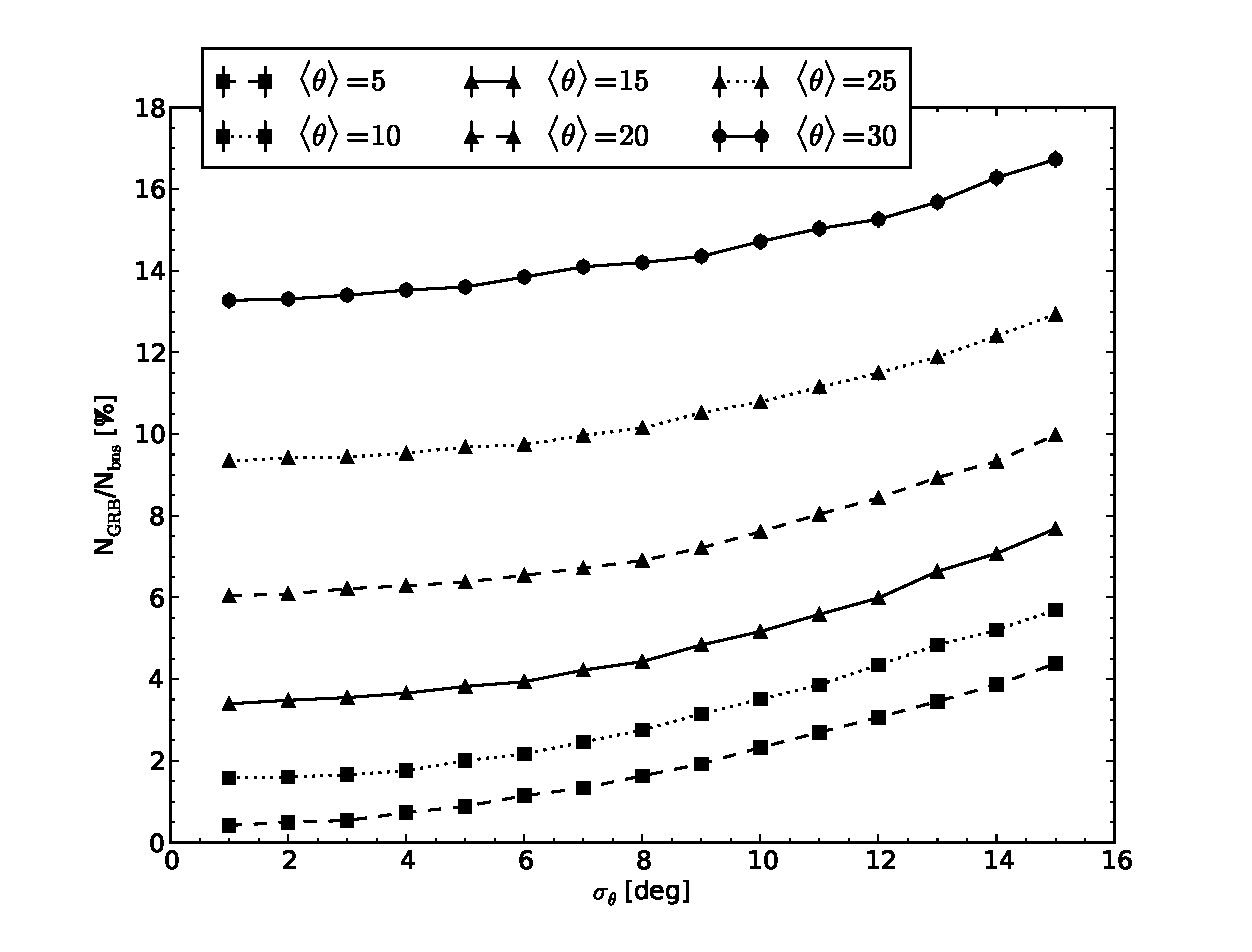
\includegraphics[width=\linewidth]{theta_dist_grbfrac.eps}
\caption{\label{fig:thetapopulation} Expected relative
numbers of observed GRBs and binary coalescences for different distributions
on the GRB beaming angle.  Lines in the figure correspond to jet angle
population means, while the $x$-axis shows the width of the distribution.  All 
distributions are Gaussian, truncated at $(0, 90]$ degrees.}
\end{figure}


\section{From Rates To Beaming Angles}

In this section, we discuss our approach to estimating the \sgrb{} beaming
angle based on the binary neutron star inspiral rate, estimated through a number
of \gw{} observations of \bns{} coalescence. We demonstrate the approach by
considering plausible detection scenarios in aLIGO.  Our ultimate goal is to
develop a generic approach that folds in uncertainties in in the binary neutron
star inspiral rate and our ignorance about the probability with which binary
neutron star inspirals actually result in \sgrb{s}.
%
An overview of the general method is as follows:

\begin{enumerate}
    \item Estimate the posterior probability distribution on the \bns{} merger rate
    in the local Universe from a number of observed gravitational wave signals
    and our knowledge of the sensitivity of the detectors.  We construct a joint
    posterior distribution on the \bns{} rate and the (unknown) probability
    $\epsilon$ that a given merger results in a \sgrb{}.
\item Use equation~\ref{eq:rate2angle}, which relates the \bns{} merger and
    \sgrb{} rates via the geometry of the beaming angle, to transform the rate
    posterior probability to a posterior probability on the mean short gamma-ray
    burst beaming angle.
\item Marginalize over $\epsilon$. We choose to consider $\epsilon$ a nuisance
    parameter because, to date, there is no accurate estimate of this parameter
    and it is not the main focus of our analysis. 
\end{enumerate}


\subsection{Constructing The Rate Posterior}
\label{sec:rate_posterior}
%   Gregory's book, `Logical Data Analysis For The Physical Sciences' has an entire
%   chapter (\S 14) devoted to `Bayesian Inference With Poisson Sampling'.  This
%   seems to match our problem rather well.  In particular, he derives expressions
%   for a Poisson rate posterior in \S 14.3, `Signal + known background' and \S
%   14.4, `Analysis of ON/OFF measurements' (``we want to infer the source rate, s,
%   when the background rate, b, is imprecisely measured'').
%
%It's tempting to jump straight into the On/off measurement stuff in \S~14.4 of
%Gregory, where the construction of the rate posterior includes the raw
%measurements of background rate.  I actually think this over-complicates things;
%if we wanted to do follow that procedure, we have to figure out the expected FAR
%for a given size of template bank etc.  There's a pretty well-established
%procedure for measuring this number: time-slides.  In fact, we don't even have
%to do any analysis.  Figure 3 (left panel) from the observing scenarios paper
%tells us everything we need to know.  Specifically, the following sentance has
%the information we need:

Our goal is to infer the posterior probability distribution for the mean \sgrb{}
beaming angle $\theta$ from \gw{} constraints on the rate of \bns{} coalescence
$\cbcrate$.  The core ingredient to the analysis then, is the posterior
probability distribution on the coalescence rate $p(\cbcrate|D,I)$, where $D$
represents some \gw{} observation and $I$ denotes other unenumerated prior
information.   To begin we will demonstrate how $p(\cbcrate|D,I)$ may be
constructed given a variety of the projected observation scenarios using aLIGO
which are described in~\cite{ade_prospects}.  Later, in
section~\ref{sec:beaming_limits} where we extend the analysis to place upper
limits on $\theta$ from the initial detector era, we consider the rate posterior
yielded by previous \gw{} analyses.

To form the posterior on the coalescence rate, we begin by constructing the
posterior on the \emph{signal} rate.  Note that these are not identical since
only those \bns{} mergers which occur within a certain range yield a detectable
signal.  Assume we have a data analysis pipeline (e.g.,
{\tt FINDCHIRP}~\cite{2012PhRvD..85l2006A}) which, when applied to the data from
our instrument, results in discrete `events' which are characterized by network
signal-to-noise ratio $\rho_c$ and which correspond to the potential
detection of an inspiral \gw{} signal from \bns{} coalescence.  The measured
rate $r$ of these events consists of two components, one due to the signals of
interest $s$, and the other a background rate $b$, which arises due to random
chance and, more importantly, instrumental and terrestrial disturbances:
%
\begin{equation}
r = s + b
\begin{cases}
s = \text{signal rate} \\
b = \text{background rate}.
\end{cases}
\end{equation}
%
Typically for an all-sky, all-time analysis, a threshold $\rho_c\geq 12$ is
applied to the events arising from the pipeline such that
$b=10^{-2}$\,yr$^{-1}$~\cite{ade_prospects}.  Since the background rate $b$ is
known then, we are just left with the problem of inferring the signal rate $s$.
Assuming a uniform prior on $s$ and a Poisson process underlying the events, it
may be shown (e.g.,~\cite{2010blda.book.....G}) that the posterior for the
signal rate, given a known background rate $b$ and $n$ events observed over a
time period $T$ is,
%
\begin{equation}
p(s|n,b,I) = C \frac{ T\left[(s+b)T\right]^n e^{-(s+b)T}}{n!},
\end{equation}
%
where,
\begin{eqnarray}
C^{-1} & = &\frac{e^{-bT}}{n!} \int_0^{\infty}\diff(sT)(s+b)^n T^n e^{-sT}\\
& = & \sum_{i=0}^n \frac{ (bT)^i e^{-bT}}{i!}.
\end{eqnarray}
%
Finally, we can transform the posterior on the \emph{signal} rate to the
underlying \emph{coalescence} rate via our knowledge of the sensitivity of the
\gw{} analysis.  In particular,  the signal detection rate is simply the product
of the intrinsic coalescence rate $\cbcrate$ and the number of \bns{} mergers
which would result in a \gw{} signal with $\rho_c\geq12$.   Expressing the
binary coalescence rate in terms of the number of mergers per \mweg{}, per year
then we require the number of galaxies $N_{\mathrm{G}}$ which may be probed by
the \gw{} analysis.  At large distances, this is well approximated at large
distances by~\cite{rates_paper},
%
\begin{equation}
    N_G = \frac{4}{3} \pi \left( \frac{\dhor}{\textrm{Mpc}}
\right)^3 (2.26)^{-3} (0.0116),
\end{equation}
%
where $\dhor$ is the horizon distance; the distance at which an
optimally-oriented \bns{} merger yields $\rho_c\geq12$, the factor of 2.26
results from averaging over sky-locations and orientations and $1.16\times
10^{-2}$\,Mpc$^{-3}$ is the extrapolated density of \mweg{} in space.

Finally, the posterior on the binary coalescence rate $\cbcrate$ is obtained from
a trivial transformation of the posterior on the signal rate $s$,
%
\begin{eqnarray}
    p(\cbcrate|n,T,b,\dhor) & = & p(s|n,T,b) \left|\frac{\diff s}{\diff \cbcrate}\right| \\
                                   & = & N_G(\dhor)p(s|n,T,b).
\end{eqnarray}
%
We see then that in this approach, the rate posterior depends only on the number
of signal detections $n$, the observation time $T$, the background rate $b$ and
the horizon distance of the search $\dhor$.  It is precisely these quantities
that comprise the detection scenarios outlined in~\cite{ade_prospects}.  Before
constructing expected rate posteriors, let us outline the transformation from
rate to beaming angle.

\subsection{Constructing the beaming angle posterior}
Inferences of the GRB beaming angle are made from the posterior probability
density on the beaming angle $p(\theta|D,I)$ where, as usual $D$ indicates some
set of observations and $I$ unenumerated prior knowledge.  Our goal then, is to
transform the measured posterior probability density on the rate $\cbcrate$ to a
posterior on the beaming angle.
%
First, note that we can express the joint distribution $p(\theta, \epsilon|D,I)$
as a Jacobian transformation of the joint distribution $p(\cbcrate,
\epsilon|D,I)$:
\begin{equation}
p(\theta,\epsilon) = p(\cbcrate,\epsilon)
\left\lvert\left\lvert
\frac{\partial(\cbcrate,\epsilon)}{\partial(\theta,\epsilon)}
\right\rvert\right\rvert,
\end{equation}
%
where we have dropped conditioning statements for notational convenience.  The
Jacobian determinant is can be  computed from equation~\ref{eq:rate2angle}.  It
is then straightforward to marginalize over $\epsilon$ to yield the posterior
on $\theta$ itself:
%
\begin{eqnarray}
    \label{eq:beam_posterior}
    p(\theta) & = & \int_{\epsilon} p(\theta,\epsilon)~\diff \epsilon\\
              & = & \int_{\epsilon} p(\cbcrate,\epsilon)
    \left\lvert\left\lvert
    \frac{\partial(\cbcrate,\epsilon)}{\partial(\theta,\epsilon)}
    \right\rvert\right\rvert~\diff \epsilon \\
              & = & \frac{2\grbrate \sin
\theta~p(\cbcrate)}{(\cos\theta-1)^2}\int_{\epsilon}
\frac{p(\epsilon)}{\epsilon} ~\diff \epsilon,
\end{eqnarray}
%
where we have assumed $\epsilon$ and $\cbcrate$ are logically independent such
that,
\begin{equation}
p(\epsilon,\cbcrate) = p(\epsilon|\cbcrate)p(\cbcrate) = p(\epsilon)p(\cbcrate).
\end{equation}
%
It is important note here that the entire procedure of deriving the jet angle
posterior is completely independent of the approach used to derive the rate
posterior. In the preceeding section we adopted a straightforward Bayesian
analysis of a Poisson rate which is amenable to a simple application of plausible
future detection scenarios; there is no inherent requirement to use that method
to derive the rate posterior.

Given the posterior on the rate $p(\cbcrate)$ then, the final ingredient in this
approach is the specification of some prior distribution for $\epsilon$.  In
this work, we will present results using three different priors:
%
\begin{description}
\item [Delta-function] $p(\epsilon) = \delta(\epsilon=0.5)$;
        the probability that \bns{} mergers yield \sgrb{s} is known to be 50\%
        exactly.

\item [Uniform] $p(\epsilon)=U(0,1)$;
        the probability that \bns{} mergers yield \sgrb{s} may lie anywhere
    $\epsilon \in (0,1]$ with equal support in that range. 

    \item [Jeffreys] $p(\epsilon)=\beta(\frac{1}{2},\frac{1}{2})$; treating the
        outcome of a \bns{} merger as a Bernoulli trial in which a \sgrb{}
        constitutes `success' and $\epsilon$ is the probability of that success,
        the least informative prior, as derived from the square root of the
        determinant of the Fisher information for the Bernoulli distribution, is
        a $\beta$-distribution with shape parameters $\alpha=\beta=\frac{1}{2}$.
\end{description}

%   \begin{figure}%[ht]
%   \centering
%   {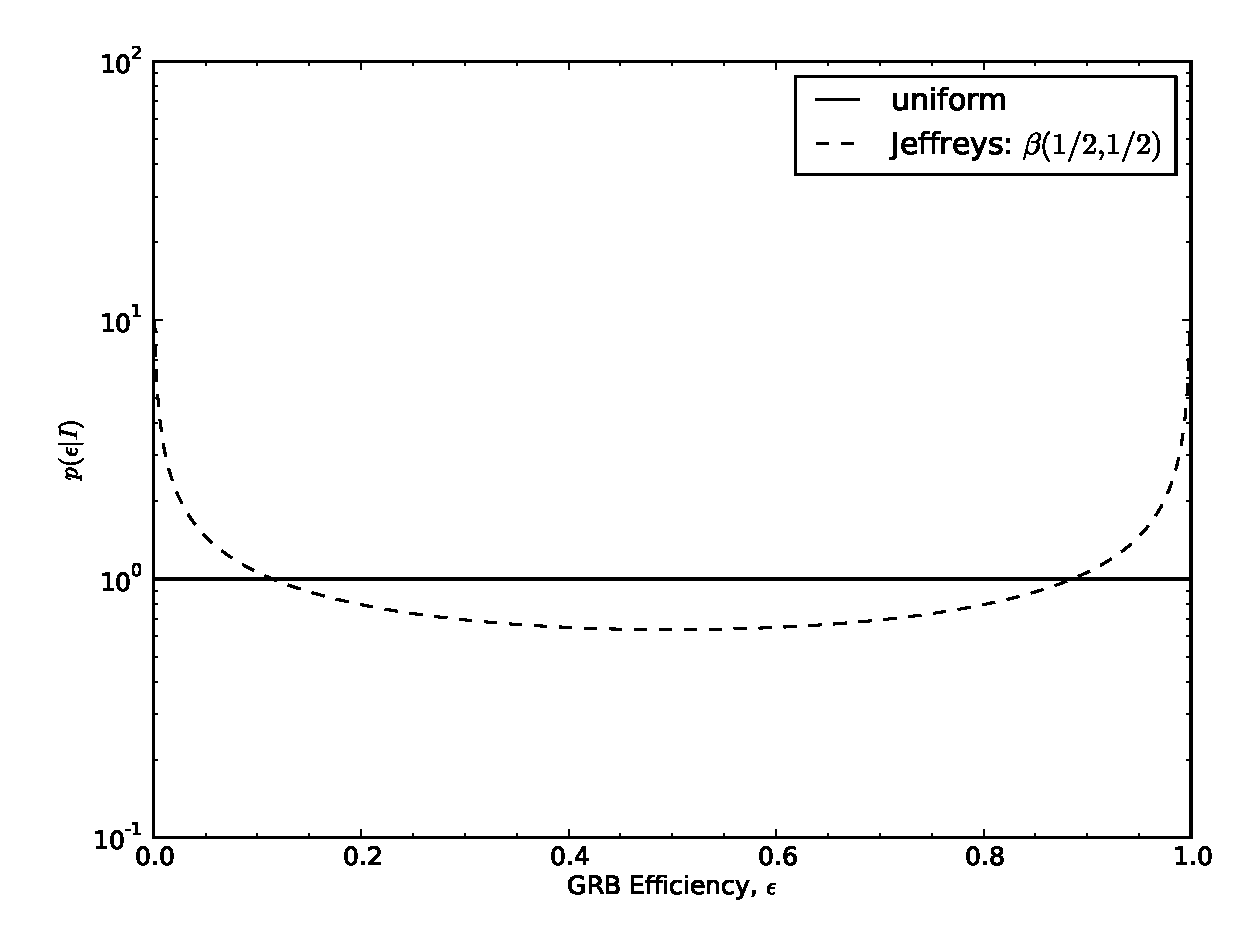
\includegraphics[width=\linewidth]{efficiency_prior.eps}}\label{fig:priors}
%   \caption{Priors}
%   \end{figure}

\section{Prospects For Beaming Angle Constraints With aLIGO}
We now demonstrate the derivation of the rate posterior $p(\cbcrate)$ and the
subsequent transformation to the beaming angle posterior $p(\theta)$.  We
consider four \gw{} observation scenarios with aLIGO based on the work
in~\cite{ade_prospects}.  An observing scenario essentially consists of an epoch
of aLIGO operation, which defines an expected search sensitivity (i.e., \bns{}
horizon distance $\dhor$) and observation time $T$; as well as an assumption on
the rate of \bns{} coalescence in the local Universe.  Each observing scenario
ultimately results in an expectation for the number of observed \gw{s} from
\bns{} coalescence. For this study, we
consider two operation epochs: the 2016 and 2022+ scenarios described
in~\cite{ade_prospects}. For each epoch we produce results for the `realistic'
and `high' \bns{} rates described in~\cite{rates_paper}.

Our first goal is to establish the expected number of detections in each
scenario. Given the observation time and horizon distance of the observation
epoch we first compute the volume accessible to the analysis,
%
\begin{equation}
    \label{eq:search_volume}
    V_{\mathrm{search}} = \frac{4}{3}\pi \left(\frac{\dhor}{2.26}\right)^3 \times \gamma T,
\end{equation}
%
where the factor 2.26 arises from averaging over source sky location and
orientation, $T$ is the observation time and $\gamma$ is the \emph{duty cycle}
for the science run.  Following~\cite{ade_prospects}, we take $\gamma=0.5$.
Where there is a range in the horizon distances quoted in~\cite{ade_prospects}
to account for uncertainty in the sensitivity of the early configuration of the
detectors, we use the arithmetic mean of the lower and upper bounds on when
computing the search volume. Table~\ref{table:scenarios} lists the details of
each observing scenario.


\begin{table}
\centering
\begin{tabular}{l c c c c c }
\toprule
Epoch & $T$ & $\dhor$ &
$\langle V_{\mathrm{search}}\rangle$ & $\cbcrate$ & $n$ \\
 & [yr] & [Mpc] & [Mpc$^3$yr] &  [Mpc$^{-3}$yr$^{-1}$] \\
\colrule
2016 & 0.5 & 80--120 & $1.05\times10^6$ & $10^{-6}$ & 1.3 \\
2016 & 0.5 & 80--120 & $1.05\times10^6$ & $10^{-5}$ & 13 \\
2022+ & 1 & 200 & $4\times10^7$ & $10^{-6}$ & 40 \\
2022+ & 1 & 200 & $4\times10^7$ & $10^{-5}$ & 400 \\
\botrule
\end{tabular}
\caption{Advanced detector era observing scenarios considered in this work.  $T$
is the expected duration of the science run and $\dhor$ is the BNS
horizon distance for the sensitivity expected to be acheived at the given epoch.
$\langle V_{\mathrm{search}}\rangle $ is the sensitive volume of the search,
where the angled brackets $\langle \rangle$ indicate averaging over the range
in horzizon distance, $\cbcrate$ is the assumed BNS coalescence rate and
$n$ is the expected number of \gw{} detections.  Note that the
quoted search volume accounts for a network duty cycle of $\sim 50\%$.
Full details may be foud in~\cite{ade_prospects}.\label{table:scenarios}}
\end{table}
%

\subsection{Posterior Results}
Figure~\ref{fig:aligorate} shows the rate posteriors resulting from the
observations described in table~\ref{table:scenarios} for the expected early
aLIGO sensitivity in the 2016 epoch (broad, solid curve) and the nominal design
sensivity (narrow, dashed curve), using the `realistic' rate
$\cbcrate=10^{-6}$\,Mpc$^{-3}$yr$^{-1}$\footnote{The curves corresponding to the
`high' rate show similar qualitative behaviour and are not included here in the
interests of brevity.}.  We now use curves such as these together with the prior
distributions described in section~\ref{sec:rate_posterior} and the observed
rate of \sgrb{s} (as described in section~\ref{sec:sgrbs}, we use
$\grbrate=10$\,Gpc$^{-3}$yr$^{-1}$~\cite{nakar-2007,Dietz11}) to derive the
corresponding beaming angle posteriors.

\begin{figure}
\centering
{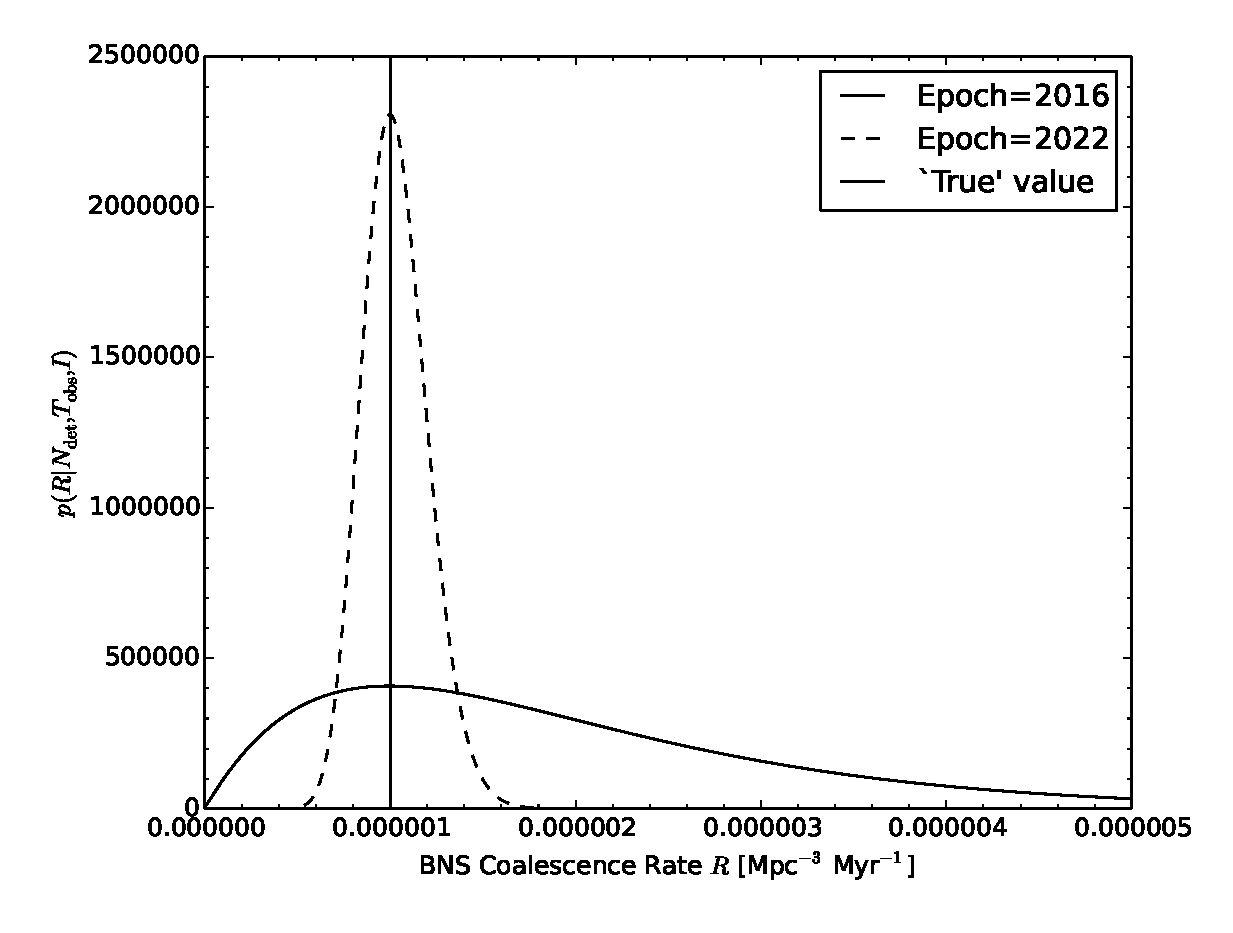
\includegraphics[width=\linewidth]{aligo_rate_re.eps}}
\caption{ADE Rate Posterior\label{fig:aligorate}}
\end{figure}

\subsubsection{Validation}
Before we go ahead and derive beaming angle posteriors corresponding to the
aforementioned observing scenarios, however, it is useful to establish some form
of validation for our procedure.  This validation is performed by first
selecting values of the beaming angle, say $\theta=30^{\circ}$; the \sgrb{}
efficiency, say $\epsilon=0.5$ and we use the `realistic' rate for the rate of
\bns{} coalescence $\cbcrate$.  We then compute the value of the \sgrb{} rate
which would correspond to these parameter choices.  Finally, we simply use this
\emph{artificial} value for $\grbrate$ in equation~\ref{eq:beam_posterior} when
we compute the posterior on the beaming angle on the understanding that the
resulting posterior should yield an inference consistent with the `true' value
$\theta=30^{\circ}$.

\begin{figure}
\centering
{\includegraphics[width=\linewidth]{jet_angle_posterior_aligo_2016.eps}}
\caption{ADE 2016 jet angle posterior, 
$\theta = 30^{\circ}$\label{fig:injjetposterio2016}}
\end{figure}

\begin{figure}
\centering
{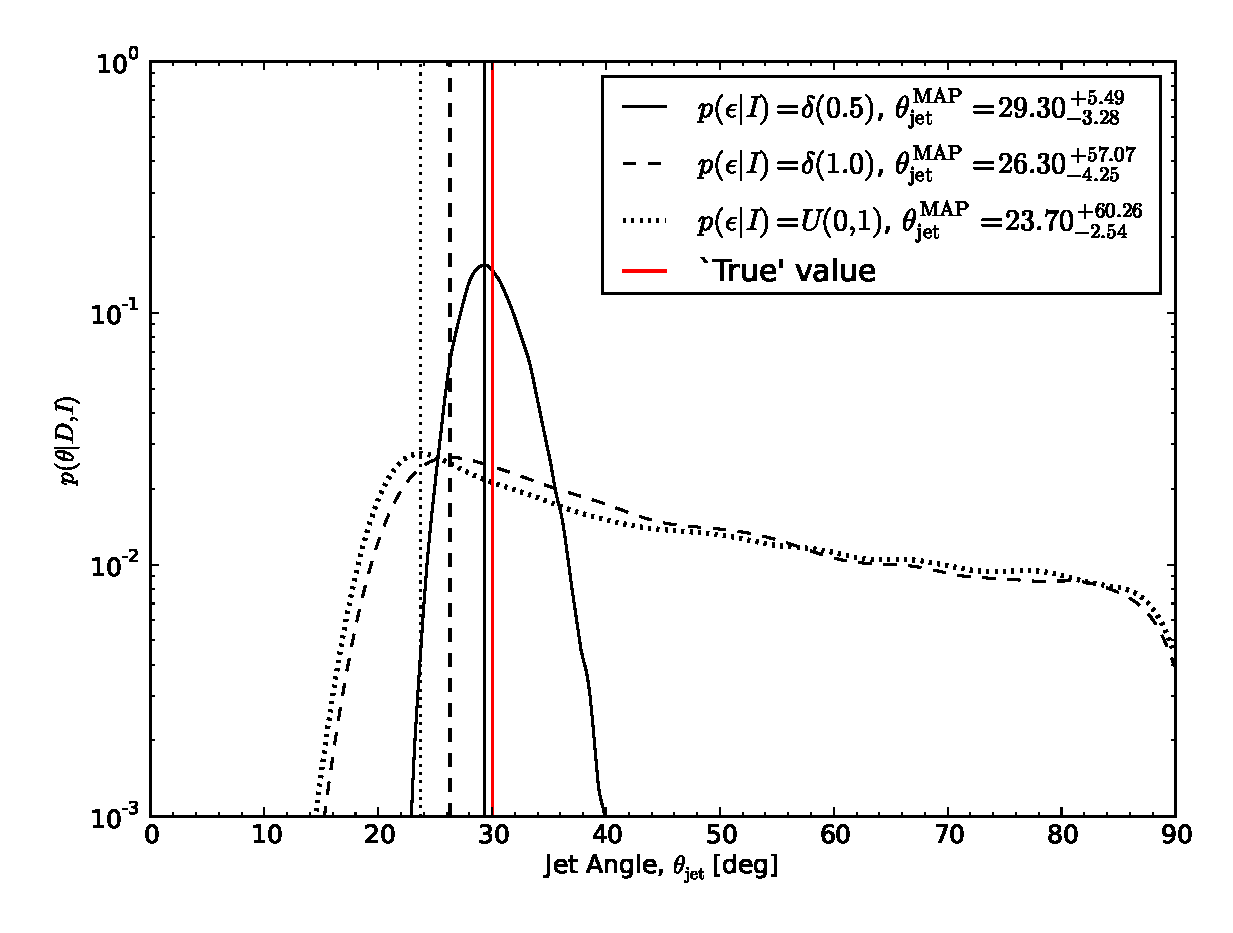
\includegraphics[width=\linewidth]{jet_angle_posterior_aligo_2022.eps}}
\caption{ADE 2022 jet angle posterior, 
$\theta = 30^{\circ}$\label{fig:injjetposterio2022}}
\end{figure}

Figures~\ref{fig:injjetposterio2016} and~\ref{fig:injjetposterio2022} show the
beaming angle posteriors which result from this analysis for the 2016 and 2022
scenarios, respectively.  Unsurprisingly, the most accurate constraints arise
when we already have the tightest possible constraints on the \sgrb{} efficiency
$\epsilon$.  That is, the beaming angle posterior arising from the
$\delta$-function prior on $\epsilon$ is the narrowest, yielding the shortest
possible confidence interval.  It is well worth remembering, however, that had
we been incorrect regarding the value of $\epsilon$ when using the
$\delta$-function prior, the result would be significantly biased and our
inference on the beaming angle would be incorrect.  This highlights the
necessity of building a suitable representation of our ignorance into the
analysis.  Finally, we note that the results from the uniform and
$\beta$-distribution priors are broadly equivalent.


\subsubsection{Jet Angle Posteriors From Observing Scenarios}

\begin{figure}
\centering
{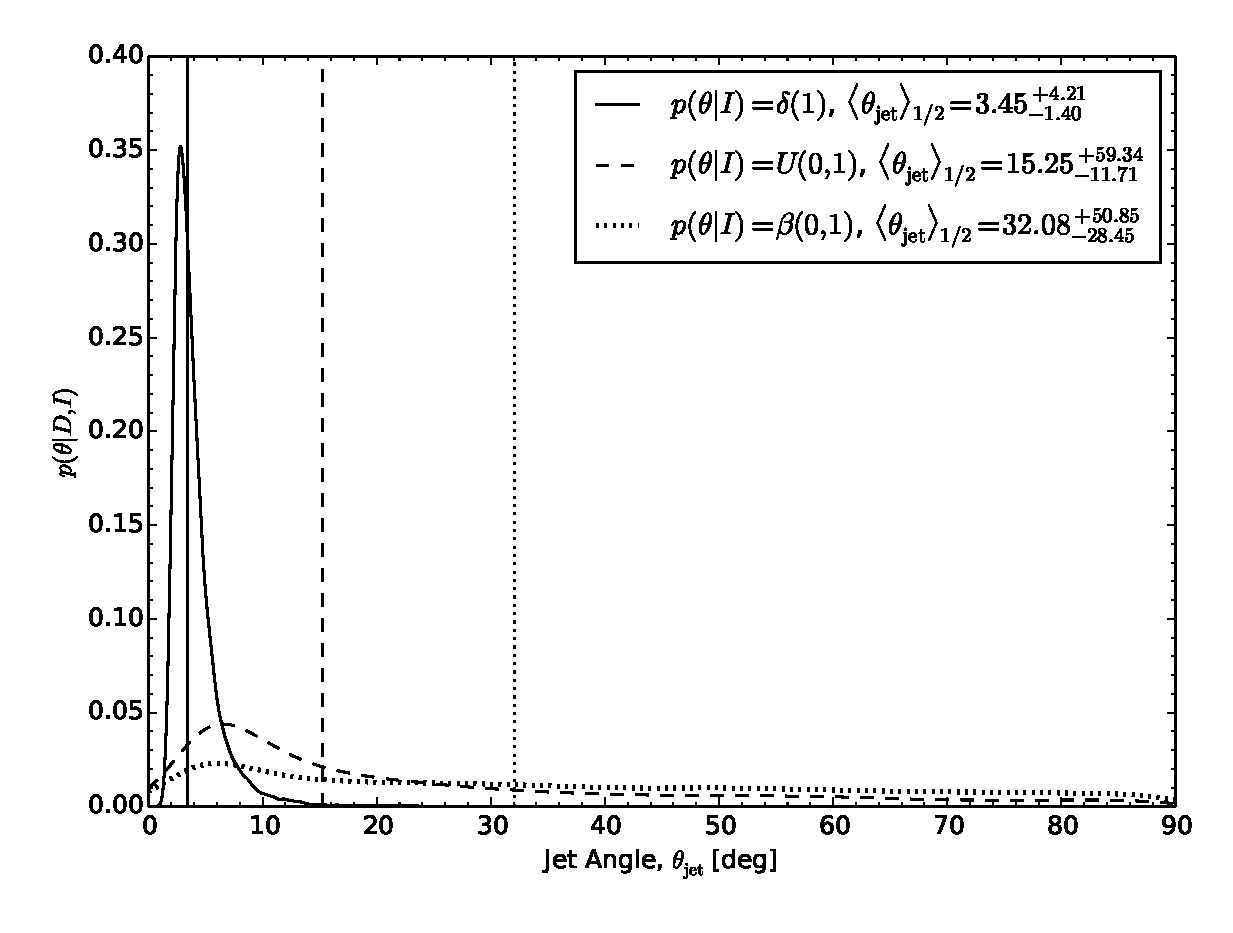
\includegraphics[width=\linewidth]{jet_angle_posterior_aligo_2016_real.eps}}
\caption{ADE 2016 jet angle posterior}
\end{figure}

\begin{figure}
\centering
{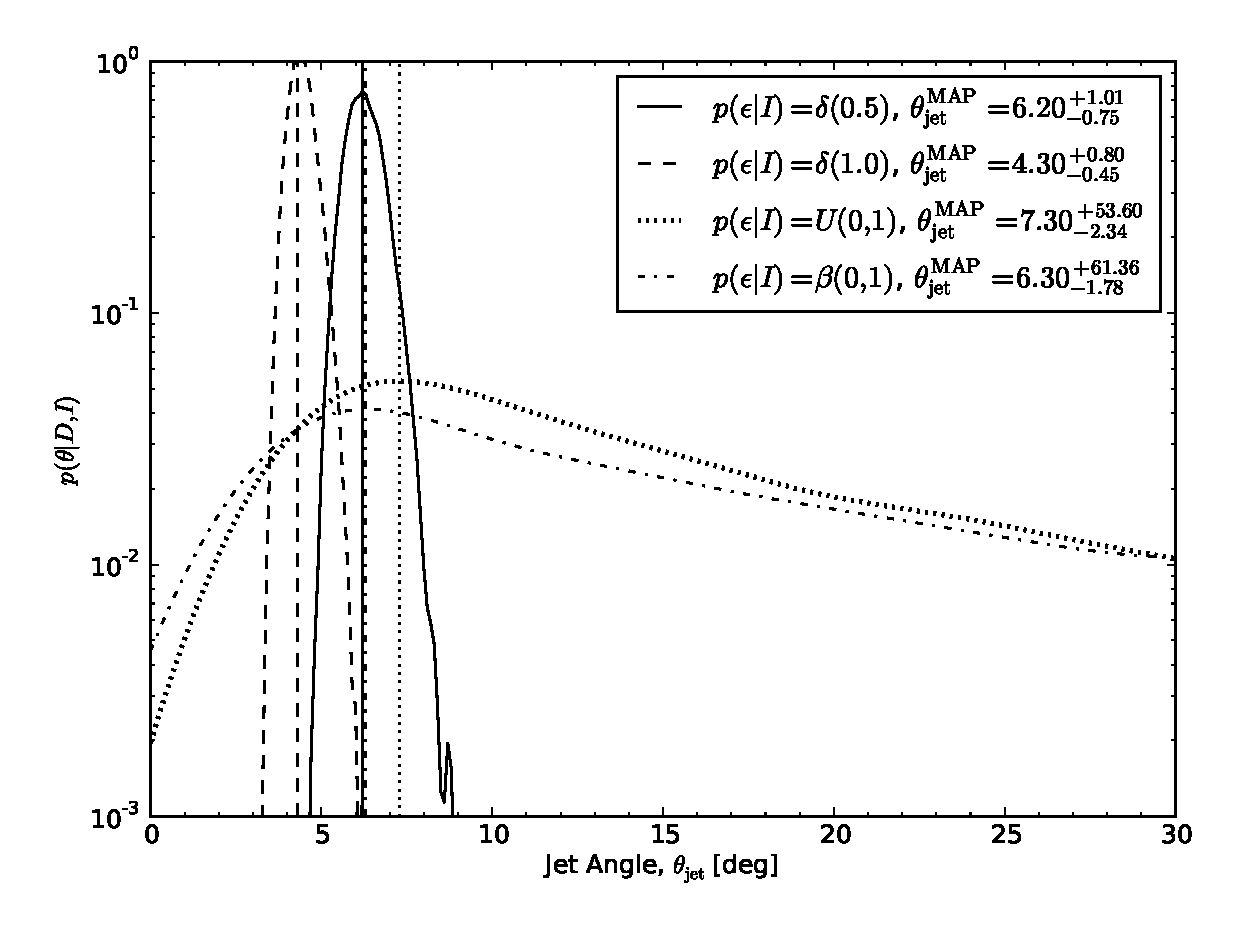
\includegraphics[width=\linewidth]{jet_angle_posterior_aligo_2022_real.eps}}
\caption{ADE 2022 jet angle posterior}
\end{figure}


\subsection{Beaming angle limits from upper limits}
\label{sec:beaming_limits}

\subsubsection{Constructing The Rate Posterior}

Our proposed approach also works if there are no observed 
gravitational wave signals from binary neutron star inspirals. In the 
case where no signals are observed, an upper limit on the binary
neutron star inspiral rate is used in place of the rate posterior 
previously described in subsection XXX.

Following~\cite{Biswas09,BradyFairhurst08}, the posterior on the binary
coalescence rate may be determined from the loudest event in the \gw{}
analysis.  Specifically, for a foreground event rate due to  binary coalescence
$\cbcrate$, the probability of obtaning no events with ranking statistic $\rho$
greater than the observed loudested event $\rhostar$ is,
%
\begin{equation}
P_F(\rhostar | \cbcrate, C_L, T) = e^{-\cbcrate C_L(\rhostar) T},
\end{equation}
%
where $C_L(\rhostar)$ is the total luminosity to which the search is sensitive
and $T$ is the duration of the search.  The overall probability of obtaining
no events with ranking statistic $\rho>\rhostar$ is the product of obtaining
no such events from foreground \emph{and} the probability of obtaining no such
events from the background in the detector, denoted $P_B(\rhostar)$,
%
\begin{equation}
P(\rhostar|\cbcrate,I) = P_B(\rhostar|I)e^{-\cbcrate C_L(\rhostar) T}
\end{equation}
%
Using a uniform prior on $\cbcrate$ and inverting the overall probability with
Bayes' theorem, we arrive at,
%
\begin{equation}\label{eq:loudestEventPosterior}
p(\cbcrate | C_L({\rhostar}), T, \Lambda) \propto p(\cbcrate) \left[ \frac{1+\Lambda
C_L(\rhostar) T}{1+\Lambda}\right] e^{-\cbcrate C_L(\rhostar) T}
\end{equation}
%
where $p(\cbcrate)$ is the prior probability distribution on the rate.  The
quantity $\hat{\Lambda}$ measures the relative probability of detecting an event
with ranking statistic $x$ due to \gw{s} versus the probability of an equally loud
event arising in the background distribution.  The reader is directed to
section\,3 of~\cite{BradyFairhurst08} for a full discussion of this quantity.


In this section, we focus attention on the interpretation of rate upper limits
from past \gw{} analyses.  We first reconstruct the measured posterior on the
binary coalescence rate and go on to compute the posterior and upper limit on
the sGRB beaming angle under a range of assumptions regarding the sGRB
efficiency $\epsilon$.

The upper limit on the binary coalescence rate at confidence $\alpha$ is found
by integrating the rate posterior from zero to $\alpha$.  Assuming a uniform
prior on the rate $\cbcrate$ and using the rate posterior given by
equation~\ref{eq:loudestEventPosterior}, the upper limit on the rate
$\cbcrate_{\alpha}$ is given by equation 21 in~\cite{BradyFairhurst08}:
%
\begin{equation}
1-\alpha =  e^{-\cbcrate_{\alpha} C_L(\rhostar)T)}
\left[ 
1+ \left(\frac{\Lambda}{1+\Lambda}\right) \cbcrate_{\alpha} T C_L(\rhostar)
\right ].
\label{eq:rateIntegral}
\end{equation}
%
In the event that no \gw{} signal has been observed and the loudest event is
umabiguously due to background noise fluctuations, we are in the limit in which
$\Lambda \rightarrow 0$.  In this case, we simply have,
\begin{equation}
C_L(\rhostar)T = -\frac{\log(1-\alpha)}{\cbcrate_{\alpha}},
\end{equation}
%
and the value of $\cbcrate$ can be taken straight from the literature\footnote{Note
that this procedure necessarily confines our jet angle inferences based on
progenitor systems for which the rate upper limits are available.  Given that
the binary coalesence rate limits are quoted for canonical binary neutron star
and neutron star-black hole systems, both plausible sGRB progenitors, this
simply means our inferences on the jet angle are specific to each system and
treated separately.}

Using the most stringent 90\% confidence upper limit from \gw{} observations on
the rate of binary neutron star coalescences to date, $\cbcrate^{90\%}_{{\rm
bns}} = 1.3\times 10^{-4}$\,Mpc$^{-3}$yr$^{-1}$~\cite{S6lowmass}, gives
$C_L(\rhostar)T=17712$.  Similarly, for NS-BH systems,  $\cbcrate^{90\%}_{{\rm
nsbh}} = 3.1\times 10^{-5}$\,Mpc$^{-3}$yr$^{-1}$ gives $C_L(\rhostar)T=74277$.
The posteriors on the rates, assuming these values and $\Lambda=0$, are shown in
figure~\ref{fig:reconstructedRatePosterior}.  

\begin{figure}
\centering
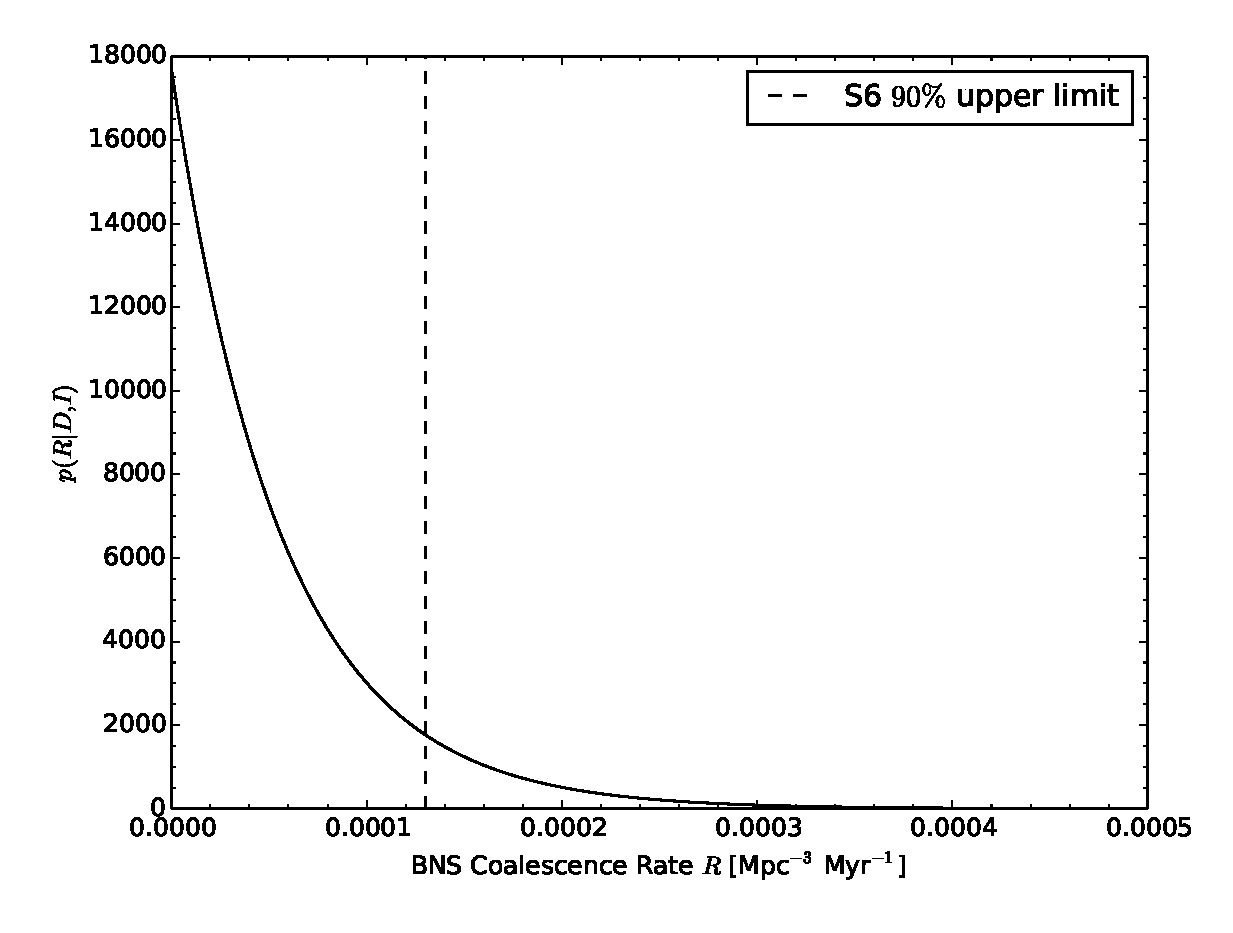
\includegraphics[width=\linewidth]{S6_rate.eps}
\caption{S6/VSR2,3 Rate Posterior\label{fig:s6rate}}
\end{figure}

\begin{figure}
\centering
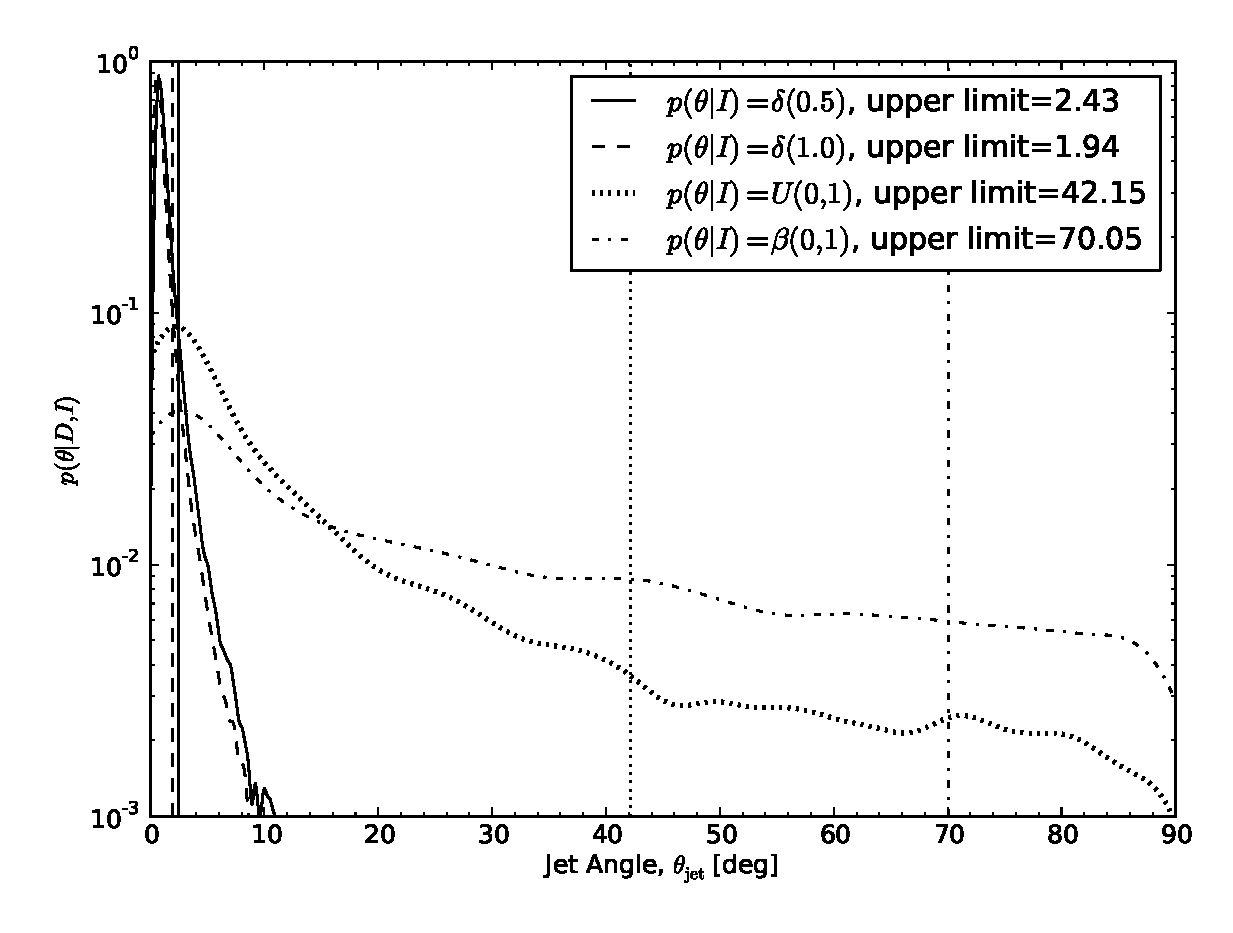
\includegraphics[width=\linewidth]{jet_angle_posterior_iligo.eps}
\caption{S6/VSR2,3 Jet Angle Posterior\label{fig:s6angle}}
\end{figure}

\section{Conclusion}

\begin{comment}

\appendix


\section{Jacobian Calculation}
This doesn't need to be in the publication, these are just notes for James'
benefit and possibly verification.

\begin{equation}
\cbcrate=\frac{\grbrate}{\epsilon(1-\cos \theta)},
\end{equation}

\begin{equation}
p(\theta) = \int_{\epsilon} p(\theta,\epsilon)~\diff \epsilon,
\end{equation}

\begin{equation}
p(\theta,\epsilon) = p(\cbcrate,\epsilon)
\left\lvert\left\lvert
\frac{\partial(\cbcrate,\epsilon)}{\partial(\theta,\epsilon)}
\right\rvert\right\rvert,
\end{equation}

% Increase matrix line spacing
\begingroup
\renewcommand*{\arraystretch}{1.5}

% matrix:
\begin{equation}
\frac{\partial (\cbcrate,\epsilon)}{\partial(\theta,\epsilon)} =
\begin{bmatrix}
\frac{\partial \cbcrate}{\partial \theta} & \frac{\partial \cbcrate}{\partial \epsilon} \\
\frac{\partial \epsilon}{\partial \theta} & \frac{\partial \epsilon}{\partial \epsilon}
\end{bmatrix}.
\end{equation}

% end line spacing increase
\endgroup

\begin{eqnarray}
\frac{\partial \cbcrate}{\partial \theta} & = &
-\frac{\grbrate\sin\theta}{\epsilon(\cos\theta - 1)^2}\\
\frac{\partial \cbcrate}{\partial \epsilon} & = &
\frac{\grbrate}{\epsilon^2(\cos\theta-1)}\\
\frac{\partial \epsilon}{\partial \theta} & = &
-\frac{\grbrate\sin\theta}{\cbcrate(\cos\theta-1)^2}\\
\frac{\partial \epsilon}{\partial \epsilon} & = & 1\\
\end{eqnarray}

\begin{eqnarray}
\left\lvert
\frac{\partial(\cbcrate,\epsilon)}{\partial(\theta,\epsilon)}
\right\rvert & = & \frac{\partial \cbcrate}{\partial \theta}
\frac{\partial \epsilon}{\partial \epsilon} - \frac{\partial \cbcrate}{\partial
\epsilon}\frac{\partial \epsilon}{\partial \theta} \\
& = & -\frac{2\sin\theta}{\epsilon(\cos\theta-1)^2}
\end{eqnarray}
%
Finally:
\begin{equation}
\left\lvert\left\lvert
\frac{\partial(\cbcrate,\epsilon)}{\partial(\theta,\epsilon)}
\right\rvert\right\rvert = \frac{2\grbrate\sin\theta}{\epsilon(\cos\theta-1)^2} 
\end{equation}

\section{Null-detection Jet Angle Posteriors With Different Priors}

\end{comment}

\bibliography{grb_beams_paper}

\end{document}
